\subsubsection{Lectura de velocidad por RS-485}

El SAL/T cuenta con tres fuentes independientes para medir la velocidad de la formación; dos de ellas provienen de una comunicación por el protocolo RS-485 con otros sistemas de la formación, la tercera proviene del módulo GPS instalado dentro del mismo SAL/T. \\ 

La fuente de medición de velocidad más confiable, y por lo tanto priorizada por el SAL/T, es la indicada por el registrador de eventos Hasler Teloc 1500. La formación cuenta con un generador de pulsos ópticos Hasler que opera en el dominio infrarrojo conectado al registrador de eventos de la formación. Al mismo tiempo, el registrador de eventos está comunicado con un indicador de velocidad que tiene disponible el maquinista \cite{indicador_velocidad}. En la figura \ref{fig:hasler_teloc} se observan los dispositivos presentes en la formación. 

\begin{figure}[H]
    \centering
    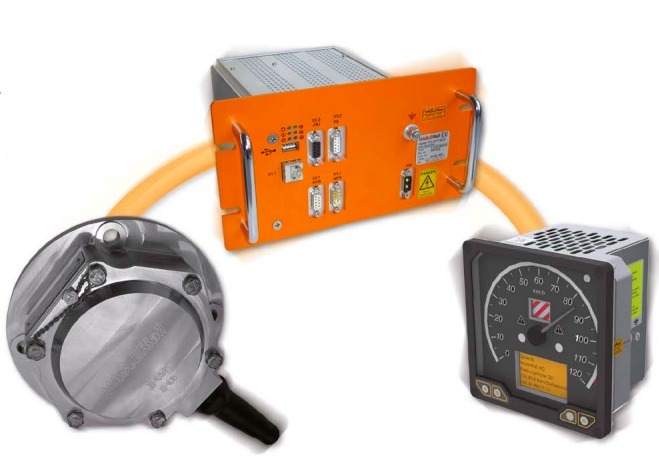
\includegraphics[width = 0.7\linewidth]{img/hasler_teloc.jpeg}
    \caption{Equipamiento Hasler en la formación ferroviaria}
    \label{fig:hasler_teloc}
\end{figure}


En el prototipo anterior del SAL/T, se realizó una tarea de ingeniería inversa para detectar cómo era la comunicación entre el registrador de eventos y el indicador de velocidad para poder interceptar esa señal y utilizar el dato de la velocidad dentro del SAL/T \cite{salt_ivan}. Revisando la documentación del equipo, con la ayuda del personal del laboratorio de material rodante de la estación de Victoria y midiendo las señales en el bus de comunicación entre estos dispositivos, se concluyó que la comunicación utilizaba el protocolo RS-485 \textit{half-duplex} a 115.200 bps. Las pruebas permitieron determinar que la señal cuadrada medida utiliza una tensión de 0,5 V para el estado bajo y de 3,3 V para el estado alto. En reposo, el bus queda en estado alto y la configuración es de 8 bits con un bit extra de stop. La trama enviada está compuesta por paquetes de 31 bytes. En la figura \ref{fig:hasler_trama} se puede observar la medición de un paquete de datos completos realizado en este proceso de descubrimiento. 

\begin{figure}[H]
    \centering
    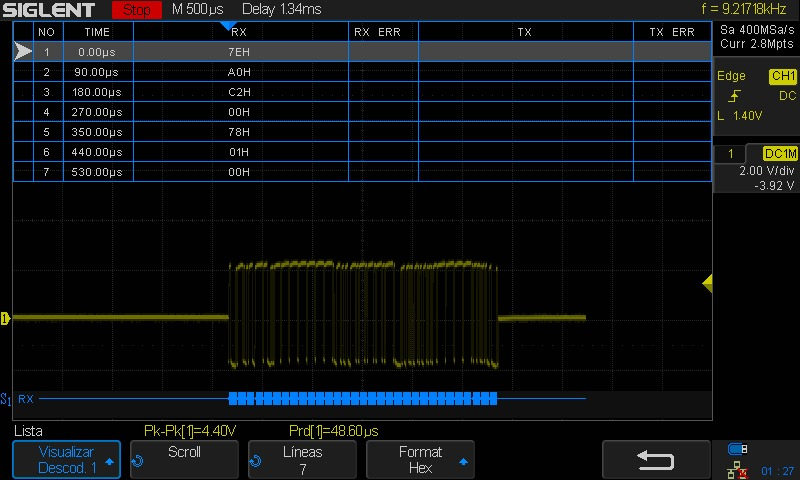
\includegraphics[width =\linewidth]{img/hasler_trama.png}
    \caption{Trama emitida por el equipo Hasler Teloc 1500}
    \label{fig:hasler_trama}
\end{figure}    

Las tramas empiezan y finalizan con un byte de start y stop, respectivamente, de valor hexadecimal 0x7E. Conociendo el byte de start y stop es más fácil aislar las tramas y analizarlas de manera independiente. Se determinó que la información asociada a la velocidad está expresada en los bytes 7 y 8 (repetida en los bytes 9 y 10) en formato hexadecimal. También, se determinó que los bytes 29 y 30 funcionan como código de redundancia cíclica en la variante CRC-16/IBM-3740 \cite{crc}. El resto de la información contenida en la trama no es relevante para el SAL/T como, por ejemplo, la cantidad de kilómetros recorridos por la formación. \\


Por otro lado, la segunda fuente de medición de velocidad por RS-485 proviene de un circuito que procesa las señales de un generador de impulsos. El generador de impulsos ópticos es un dispositivo que detecta interrupciones de un haz de luz, generalmente producido por un LED, y convierte esos cambios en señales eléctricas. Se utiliza para medir la velocidad o posición de objetos en movimiento, como ruedas o ejes, generando pulsos proporcionales a la rotación o desplazamiento. En la figura \ref{fig:pulse_generator} se puede ver el principio de funcionamiento de este dispositivo. 


\begin{figure}[H]
    \centering
    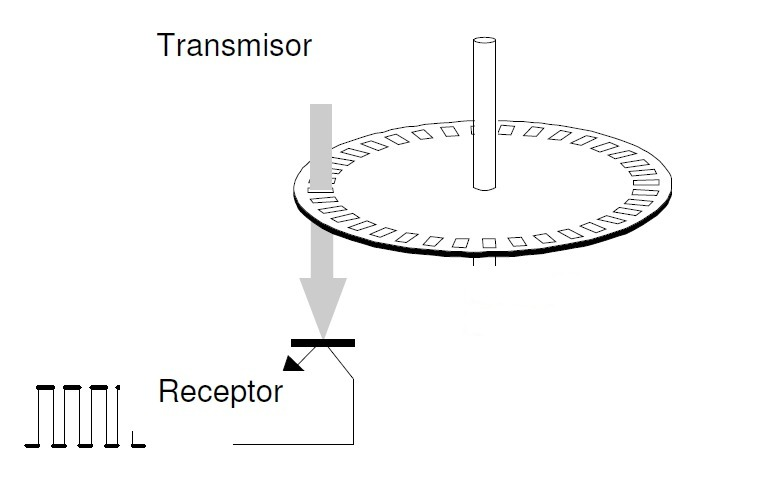
\includegraphics[width = 0.7 \linewidth]{img/pulse_generator.jpeg}
    \caption{Principio de funcionamiento de un generador de impulsos ópticos}
    \label{fig:pulse_generator}
\end{figure}    


Para determinar la velocidad a partir de la señal eléctrica, un sistema con un microcontrolador que tiene previamente configuradas algunas características del generador óptico y de la formación (números de pulsos por revolución, diámetro o circunferencia de la rueda) debe considerar la frecuencia de los pulsos así como el tiempo entre pulsos para una medición más precisa de la velocidad instantánea. Una vez determinada la velocidad, este sistema externo va a montar el dato sobre un bus RS-485 que se va a conectar con el SAL/T comunicando directamente el dato de la velocidad. \\ 


Dentro del SAL/T se incluyeron dos circuitos para realizar la conversión entre el protocolo RS-485 y las interfaces UART del MCU. Para armar este circuito, se tomó como referencia el circuito del mismo propósito incluido en la placa EDU-CIAA-NXP \cite{edu-ciaa}. El circuito está basado en el chip SN65HVD1176DR de Texas Instruments \cite{SN65HVD1176DR}; este es un  transceptor diferencial que trabaja en \textit{half-duplex} con características optimizadas para su uso en aplicaciones PROFIBUS \cite{profibus}. El voltaje diferencial de salida del controlador supera los requisitos de PROFIBUS de 2,1 V con una carga de 54 Ω. Una tasa de señalización de hasta 40 Mbps permite un crecimiento tecnológico hacia velocidades altas de transferencia de datos. La baja capacitancia del bus reduce la distorsión de la señal. \\

El circuito se muestra en la figura \ref{fig:rs485_sch} y se observa en la entrada las señales de recepción y transmisión que se conectan al MCU así como un pin de salida digital que selecciona si se van a transmitir o recibir datos ya que es un sistema \textit{half-duplex} y se comparte el bus para ambas transmisiones. Se observan también dos capacitores de desacople conectados en la alimentación del circuito integrado. Del lado de la salida se colocaron las resistencias de 390 $\Omega$ y 220 $\Omega$ conocidas como \textit{bias resistors} en las recomendaciones de PROFIBUS. Por otro lado, se colocaron los \textit{jumpers} JP6, JP7 y JP8 que deben ser cortocircuitados en caso de ser el último nodo de la red. También se colocó la resistencia R22 de 100 $\Omega$ para conectar la tierra y disipar cualquier pequeña diferencia de tensión que pueda haber entre las distintas tierras de los dispositivos conectada de acuerdo a la nota de aplicación de Texas Instruments SLLA070D \cite{rs485}; esto permite reducir el ruido de modo común en las líneas de transmisión. El circuito también utiliza el diodo supresor de transitorios (TVS) modelo SZP6SMB12CAT3G de Littelfuse \cite{SZP6SMB12CAT3G} diseñado para proteger componentes electrónicos sensibles de picos de voltaje y transitorios y el fusible reajustable MF-USMF020-2 de Bourns \cite{MF-USMF020-2} diseñado para proteger circuitos electrónicos contra sobrecorrientes. A diferencia de los fusibles tradicionales, este dispositivo puede ser reajustado manualmente después de que se ha activado, lo que proporciona una solución más conveniente y económica.




\begin{figure}[H]
    \centering
    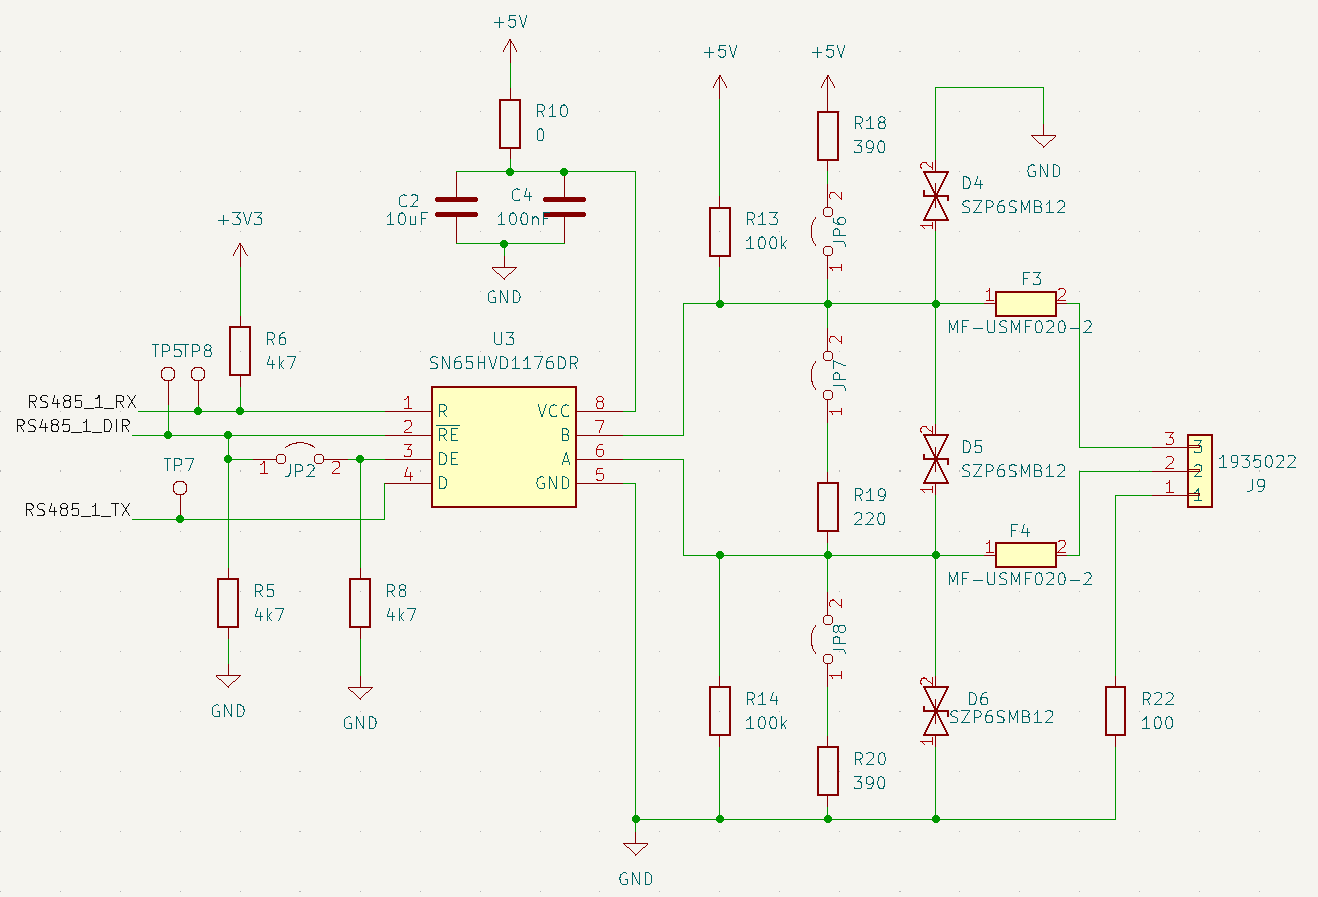
\includegraphics[width =\linewidth]{img/rs485_sch.png}
    \caption{Circuito conversor entre protocolos UART y RS-485}
    \label{fig:rs485_sch}
\end{figure}    